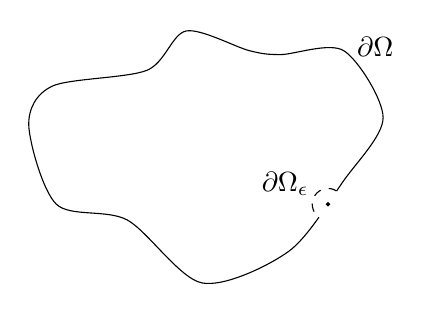
\begin{tikzpicture}
    \begin{scope}[scale = 1]
        %\draw[step = .05] (-2.5,-2) grid (2.5,2);
        \draw plot [smooth cycle] coordinates {(-2, 0) (-1.7, .5) (-.5, .7) (0, 1.2) (.8, .95) (1.2, .9) (2, .95) (2.5, .1) (2, -.7) (1.3, -1.6) (.2, -2) (-.75, -1.2) (-1.65, -1)};
        \node at (2.4, 1) {$\partial\Omega$};
        \def\initialangle{57} \def\endangle{235}
        \def\Ox{1.8} \def\Oy{-1}
        \coordinate (O) at (\Ox, \Oy);
        \draw[very thick, color = white] (O)--({\Ox + .2*cos(\initialangle)}, {\Oy + .2*sin(\initialangle)});
        \draw[very thick, color = white] (O)--({\Ox + .2*cos(\endangle)}, {\Oy + .2*sin(\endangle)});
        \draw[dashed] ({\Ox + .2*cos(\initialangle)}, {\Oy + .2*sin(\initialangle)}) arc (\initialangle:\endangle:.2);
        \draw[fill = black] (O) circle (.02) node[below right]{$\bzhe$};
        \node at ({\Ox + .6*cos(155)}, {\Oy + .6*sin(155)}) {$\partial\Omega_{\epsilon}$}; 
    \end{scope}
\end{tikzpicture}